\documentclass[12pt]{article}
\usepackage{fancyhdr}
\usepackage[letterpaper, margin=1in]{geometry}
%\usepackage{indentfirst}
\usepackage{graphicx}
\usepackage{amsmath}
\usepackage{amssymb}
\usepackage{siunitx}
\sisetup{detect-weight=true, detect-family=true} % makes siunitx follow font formatting like bold, italic, etc.
\usepackage{cancel}
\usepackage{isotope}
\usepackage{listings}
\usepackage[dvipsnames,table]{xcolor}
\usepackage{xspace}
\usepackage{booktabs} % makes tables pretty
\usepackage{longtable} % for long tables
\usepackage{multirow} % makes tables pretty
\usepackage{multicol} % makes tables pretty
\usepackage{setspace}
\usepackage{subcaption}
\usepackage{hyperref}
\usepackage{cleveref}
\newcommand{\creflastconjunction}{, and\nobreakspace} % adds oxford comma to cleveref
\usepackage[utf8]{inputenc}
\usepackage{textcomp}
\usepackage{titlesec}
\usepackage{svg}
\usepackage{pdflscape} % makes pages landscape
\usepackage{mathtools}
\usepackage{enumitem}
\usepackage[T1]{fontenc}


% ----------------- Commands ---------------------%
\newcommand{\mathcolorbox}[2]{\colorbox{#1}{$\displaystyle #2$}}
\definecolor{codegreen}{rgb}{0,0.6,0}
\definecolor{codegray}{rgb}{0.5,0.5,0.5}
\definecolor{codepurple}{rgb}{0.58,0,0.82}
\definecolor{backcolour}{rgb}{0.95,0.95,0.92}

% listings stuff for python
% Default fixed font does not support bold face
\DeclareFixedFont{\ttb}{T1}{txtt}{bx}{n}{12} % for bold
\DeclareFixedFont{\ttm}{T1}{txtt}{m}{n}{12}  % for normal

% Custom colors
%\usepackage{color}
\definecolor{deepblue}{rgb}{0,0,0.5}
\definecolor{deepred}{rgb}{0.6,0,0}
\definecolor{deepgreen}{rgb}{0,0.5,0}

%\usepackage{listings}

% Python style for highlighting
\newcommand\pythonstyle{\lstset{
language=Python,
basicstyle=\ttm,
morekeywords={self},              % Add keywords here
keywordstyle=\ttb\color{deepblue},
emph={MyClass,__init__},          % Custom highlighting
emphstyle=\ttb\color{deepred},    % Custom highlighting style
stringstyle=\color{deepgreen},
commentstyle=\color{codegray},
backgroundcolor = \color{backcolour},
breaklines=true,
numbers=left,
numberstyle=\small\color{codegray},
frame=tb,                         % Any extra options here
showstringspaces=false
}}

% Python for external files
\newcommand\pythonexternal[2][]{{
\pythonstyle
\lstinputlisting[#1]{#2}}}




% si units stuff
\DeclareSIUnit\year{yr}
\DeclareSIUnit\hour{hr}
\DeclareSIUnit\mole{mol}

% fancy header stuff
\usepackage{fancyhdr}
\pagestyle{fancy}

\setlength{\headheight}{28pt}
\lhead{NSE 565 \\ Winter 2022}
\chead{Homework 2\\}
\rhead{Austin Warren\\Due March 11, 2022}

% bib if needed
\bibliographystyle{ieeetr}

\begin{document}

%%%%%%%%%%%%%%%%%%%%%%%%%%%%%%%%%%
\section{Methods}
We will use the Upwind scheme for the spatial discretization. The conditions for the Upwind scheme are listed below:
\begin{equation}
    \phi_{i+1} = \begin{cases}
                    \phi_{I} & \overline{V} > 0\\
                    \phi_{I+1} & \overline{V} < 0
                 \end{cases}\:,
    \label{eq:upwind conditions}
\end{equation}
and
\begin{equation}
    \left(\frac{\partial \phi}{\partial x}\right)_{i-1} = \frac{\phi_{I} - \phi_{I-1}}{\Delta x}\:.
    \label{eq:cds gradient}
\end{equation}
To set up the temporal discretization, we begin with the transient convection-diffusion equation.
\begin{equation}
    \int\limits_{\Delta t}\frac{\partial}{\partial t}\left( \int\limits_{CV}\rho\phi dV \right)dt + \int\limits_{\Delta t}\:\int\limits_{S}\rho u_x \phi \cdot \overline{n}\:dS\:dt = \int\limits_{\Delta t}\:\int\limits_{S} \Gamma \frac{\partial \phi}{\partial x} \cdot \overline{n}\:dS\:dt
    \label{eq:trans conv diff}
\end{equation}
We can apply the surface integral approximations to get:
\begin{equation*}
    \int\limits_{\Delta t}\frac{\partial}{\partial t}\left( \int\limits_{CV}\rho\phi dV \right)dt + \int\limits_{\Delta t}\left[ \rho u_x S\left( \phi_{i+1} - \phi_{i-1} \right) \right]\:dt = \int\limits_{\Delta t}\Gamma S\left[ \left( \frac{\partial \phi}{\partial x} \right)_{i+1} - \left( \frac{\partial \phi}{\partial x} \right)_{i-1} \right] dt\:.
\end{equation*}
Performing the rest of the integrations, we get:
\begin{equation}
    \rho V \left( \phi_{I}^{n+1} - \phi_{I}^{n} \right) + \rho u_x S \left( \phi_{i+1} - \phi_{i-1} \right)\:\Delta t = \Gamma S \left[ \left( \frac{\partial \phi}{\partial x} \right)_{i+1} - \left( \frac{\partial \phi}{\partial x} \right)_{i-1} \right]\Delta t\:.
    \label{eq:trans disc}
\end{equation}
We can apply \Cref{eq:upwind conditions} and \Cref{eq:cds gradient} for positive velocity. We can also divide by the surface to get:
\begin{equation}
    \rho\: \Delta x \left( \phi_{I}^{n+1} - \phi_{I}^{n} \right) + \rho u_x \Delta t \left( \phi_{I}^{X} - \phi_{I-1}^{X} \right) = \Gamma\:\Delta t \left[ \left( \frac{\phi_{I+1}^{X} - \phi_{I}^{X}}{\Delta x} \right) - \left( \phi_{I}^{X} - \phi_{I-1}^{X} \right) \right]\:.
    \label{eq:trans upwind}
\end{equation}
We have three different time discretizations for this problem: Explicit Euler, Implicit Euler, and Trapezoidal. We can use \Cref{eq:trans upwind} for each scheme's inner nodes, but the boundary nodes will need to use \Cref{eq:trans disc} since they have different gradients.


\subsection{Explicit Euler}
Explicit Euler uses the substitution: $\phi^{X} = \phi^{n}$.
Inner Nodes:
\begin{equation}
    \phi_{I}^{n+1} = \left[ \frac{u_x\: \Delta t}{\Delta x} + \frac{\Gamma\: \Delta t}{\rho\: \left(\Delta x)^2\right)} \right] \phi_{I-1}^{n} + \left[ 1 - \frac{u_x\: \Delta t}{\Delta x} - \frac{2\Gamma\: \Delta t}{\rho\: \left(\Delta x\right)^2} \right] \phi_{I}^{n} + \left[ \frac{\Gamma\:\Delta t}{\rho\: \left(\Delta x\right)^2} \right]\phi_{I+1}^{n}
    \label{eq:ee inner}
\end{equation}
Left Node (Node 1): $\phi_{i-1} = \phi_L$ and $\left( \frac{\partial \phi}{\partial x} \right)_{i-1} = \frac{\phi_I - \phi_L}{\Delta x/2}$
\begin{equation}
    \phi_{I}^{n+1} = \left[ \frac{u_x\: \Delta t}{\Delta x} \right]\phi_{L} + \left[ 1 - \frac{u_x\:\Delta t}{\Delta x} - \frac{3\Gamma\:\Delta t}{\rho\left(\Delta x\right)^2} \right]\phi_{I}^{n} + \left[ \frac{\Gamma\:\Delta t}{\Delta x} \right]\phi_{I+1}^{n}
    \label{eq:ee left}
\end{equation}
Right Node (Node N): $\phi_{i+1} = \phi_R$ and $\left( \frac{\partial \phi}{\partial x} \right)_{i+1} = \frac{\phi_R - \phi_I}{\Delta x/2}$
\begin{equation}
    \phi_{I}^{n+1} = \left[ \frac{u_x\:\Delta t}{\Delta x} + \frac{\Gamma\:\Delta t}{\rho\left(\Delta x\right)^2} \right]\phi_{I-1}^{n} + \left[ 1 - \frac{u_x\:\Delta t}{\Delta x} - \frac{3\Gamma\:\Delta t}{\rho\left(\Delta x\right)^2} \right]\phi_{I}^{n} + \left[ \frac{2\Gamma\:\Delta t}{\rho\left(\Delta x\right)^2} \right]\phi_{R}
    \label{eq:ee right}
\end{equation}


\subsection{Implicit Euler}
Implicit Euler uses the substitution: $\phi^{X} = \phi^{n+1}$.
Inner Nodes:
\begin{equation}
    \left[ \frac{-u_x\: \Delta t}{\Delta x} - \frac{\Gamma\:\Delta t}{\rho\left(\Delta x\right)^2} \right]\phi_{I-1}^{n+1} + \left[ 1 + \frac{u_x\: \Delta t}{\Delta x} + \frac{2\Gamma\: \Delta t}{\rho\left(\Delta x\right)^2} \right]\phi_{I}^{n+1} + \left[ -\frac{\Gamma\: \Delta t}{\rho\left(\Delta x\right)^2} \right]\phi_{I+1}^{n+1} = \phi_{I}^{n}
    \label{eq:ie inner}
\end{equation}
Left Node (Node 1): $\phi_{i-1} = \phi_L$ and $\left( \frac{\partial \phi}{\partial x} \right)_{i-1} = \frac{\phi_I - \phi_L}{\Delta x/2}$
\begin{equation}
    \left[ 1 + \frac{u_x\:\Delta t}{\Delta x} + \frac{3\Gamma\:\Delta t}{\rho\left(\Delta x\right)^2} \right]\phi_{I}^{n+1} + \left[ -\frac{\Gamma\:\Delta t}{\rho\left(\Delta x\right)^2} \right]\phi_{I+1}^{n+1} = \phi_{I}^{n} + \left[ \frac{u_x\:\Delta t}{\Delta x} + \frac{2\Gamma\:\Delta t}{\rho\left(\Delta x\right)^2} \right]\phi_{L}
    \label{eq:ie left}
\end{equation}
Right Node (Node N): $\phi_{i+1} = \phi_R$ and $\left( \frac{\partial \phi}{\partial x} \right)_{i+1} = \frac{\phi_R - \phi_I}{\Delta x/2}$
\begin{equation}
    \left[ -\frac{u_x\:\Delta t}{\Delta x} - \frac{\Gamma\:\Delta t}{\rho\left(\Delta x\right)^2} \right]\phi_{I-1}^{n+1} + \left[ 1 + \frac{u_x\:\Delta t}{\Delta x} + \frac{3\Gamma\:\Delta t}{\rho\left(\Delta x\right)^2} \right]\phi_{I}^{n+1} = \phi_{I}^{n} + \left[ \frac{2\Gamma\:\Delta t}{\rho\left(\Delta x\right)^2} \right]\phi_{R}
    \label{eq:ie right}
\end{equation}


\subsection{Trapezoidal}
\begin{multline*}
    \left[ -\frac{\rho u_x\: \Delta t}{2} - \frac{\Gamma\: \Delta t}{2\: \Delta x} \right]\phi_{I-1}^{n+1} + \left[ \rho \:\Delta x + \frac{\rho u_x\: \Delta t}{2} + \frac{\Gamma\: \Delta t}{\Delta x} \right]\phi_{I}^{n+1} + \left[ -\frac{\Gamma\: \Delta t}{2\: \Delta x} \right]\phi_{I+1}^{n+1}\\
    = \left[ \frac{\rho u_x\: \Delta t}{2} + \frac{\Gamma\: \Delta t}{2\: \Delta x} \right]\phi_{I-1}^{n} + \left[ \rho \:\Delta x - \frac{\rho u_x\: \Delta t}{2} - \frac{\Gamma\: \Delta t}{\Delta x} \right]\phi_{I}^{n} + \left[ \frac{\Gamma\: \Delta t}{2\: \Delta x} \right]\phi_{I+1}^{n}
\end{multline*}



\clearpage
\section{Results}

\subsection{Explict Euler}
\Cref{fig:ee1,,fig:ee2,,fig:ee3} show the results for the Explicit Euler solution using $K=0.2,2.0$, and 20.0, respectively. \Cref{tab:error ee} shows the norm error for all Explicit Euler cases.
\begin{figure}[htbp]
    \centering
    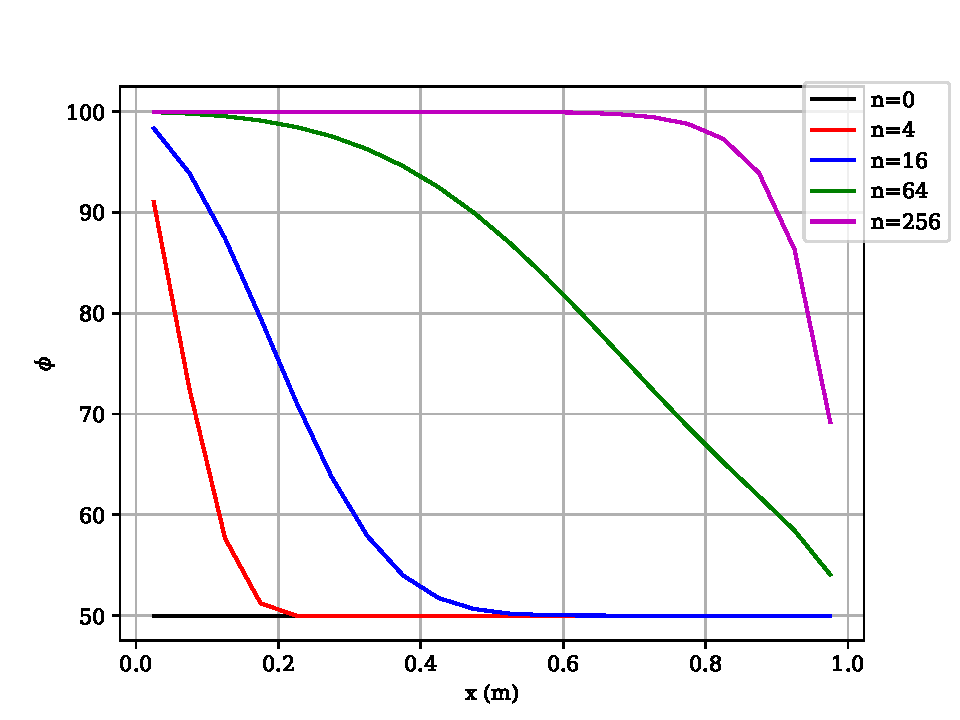
\includegraphics[width=\textwidth]{plots/graph_EE_case1.pdf}
    \caption{Explicit Euler solution for case 1: $K=0.2$.}
    \label{fig:ee1}
\end{figure}

\begin{figure}[htbp]
    \centering
    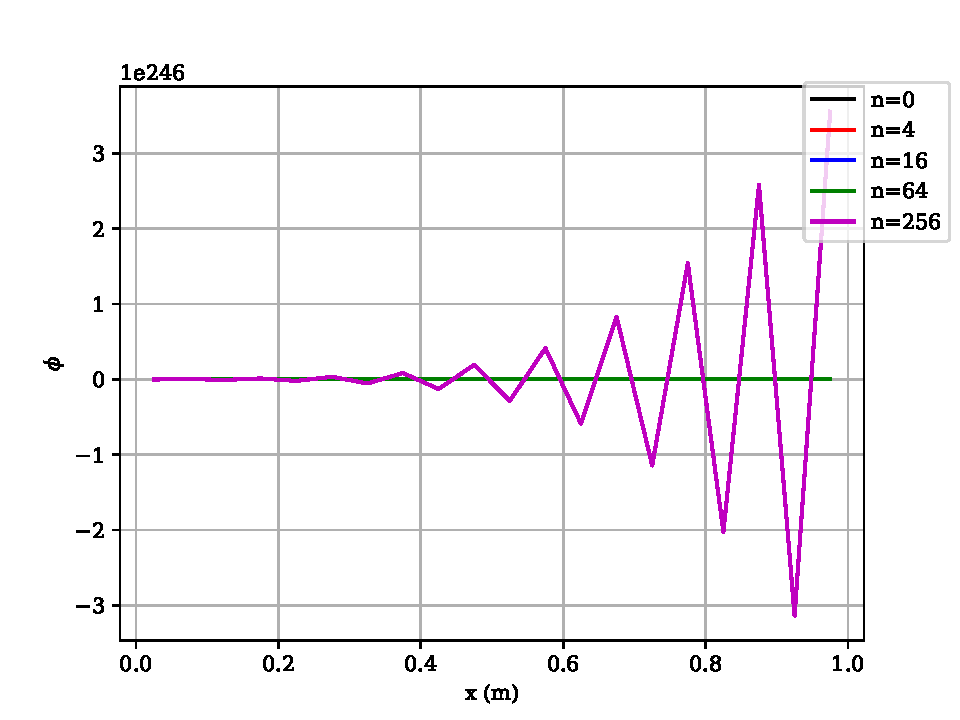
\includegraphics[width=\textwidth]{plots/graph_EE_case2.pdf}
    \caption{Explicit Euler solution for case 2: $K=2.0$.}
    \label{fig:ee2}
\end{figure}

\begin{figure}[htbp]
    \centering
    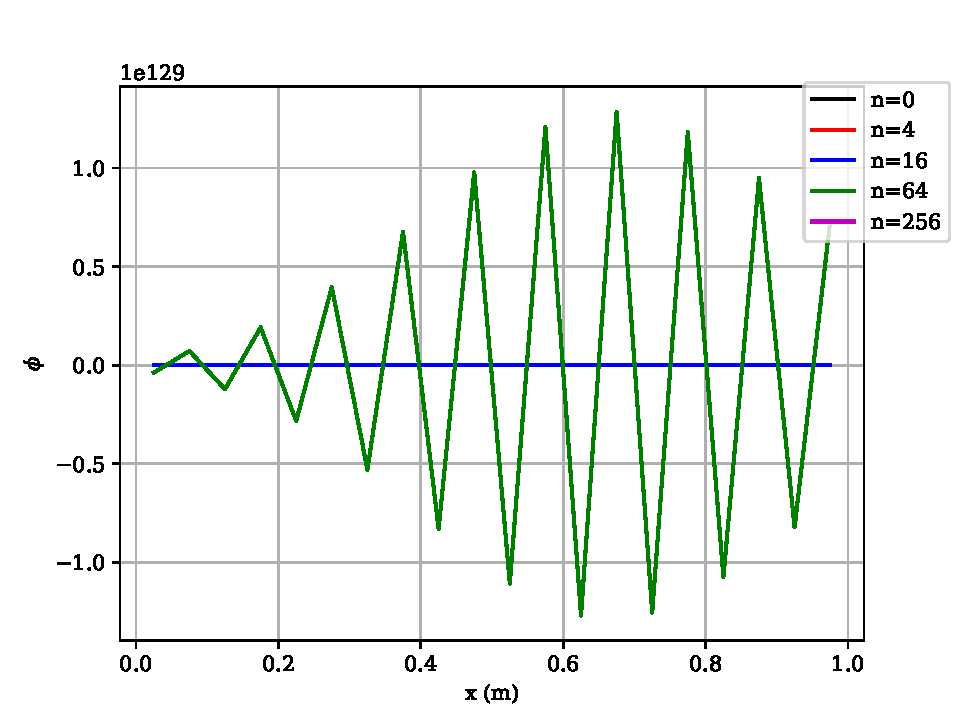
\includegraphics[width=\textwidth]{plots/graph_EE_case3.pdf}
    \caption{Explicit Euler solution for case 3: $K=20.0$.}
    \label{fig:ee3}
\end{figure}

Norm:
\begin{table}[htbp]
	 \centering
	 \caption{Norm values for Explicit Euler.}
	 \begin{tabular}{cc}
		 \toprule
		 $K$ & Norm \\ 
		 \midrule 
		 0.2 & 1.55418029575927 \\ 
		 2.0 & 8.3196861106867e+245 \\ 
		 20.0 & inf \\ 
		 \bottomrule 
	 \end{tabular} 
	 \label{tab:error ee} 
\end{table}


\clearpage
\subsection{Implicit Euler}
\Cref{fig:ie1,,fig:ie2,,fig:ie3} show the results for the Explicit Euler solution using $K=0.2,2.0$, and 20.0, respectively. \Cref{tab:error ie} shows the norm error for all Explicit Euler cases.
\begin{figure}[htbp]
    \centering
    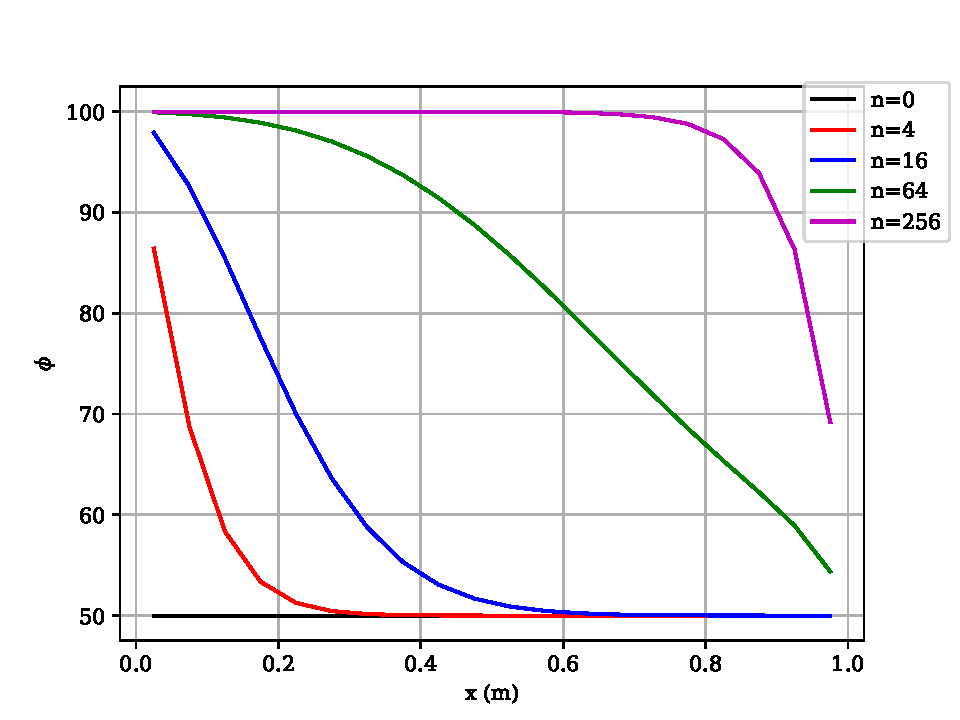
\includegraphics[width=\textwidth]{plots/graph_IE_case1.pdf}
    \caption{Implicit Euler solution for case 1: $K=0.2$.}
    \label{fig:ie1}
\end{figure}

\begin{figure}[htbp]
    \centering
    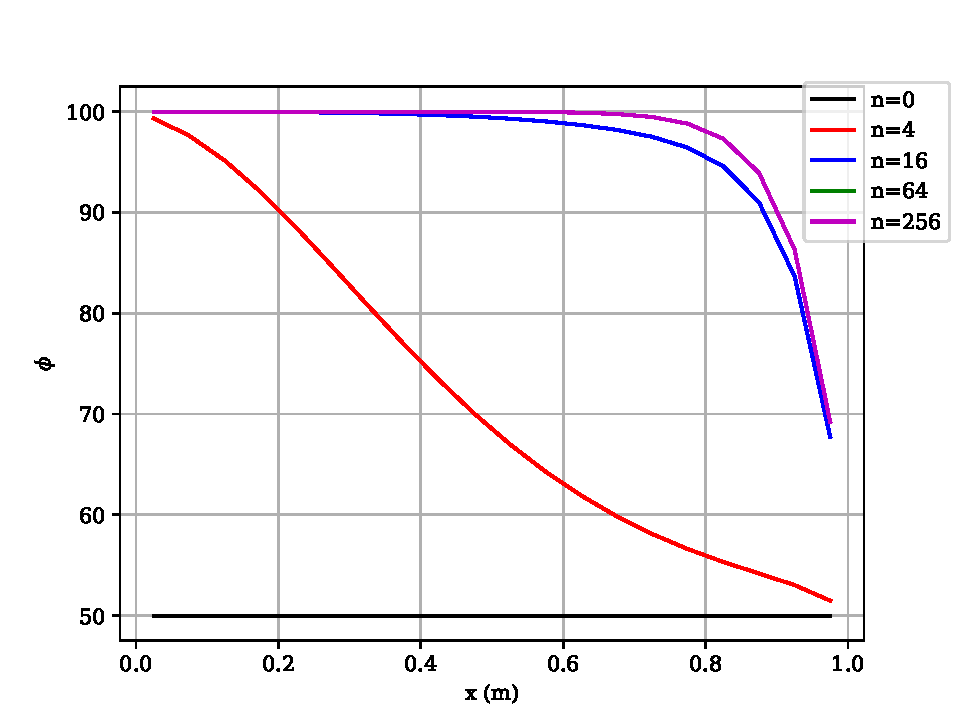
\includegraphics[width=\textwidth]{plots/graph_IE_case2.pdf}
    \caption{Implicit Euler solution for case 2: $K=2.0$.}
    \label{fig:ie2}
\end{figure}

\begin{figure}[htbp]
    \centering
    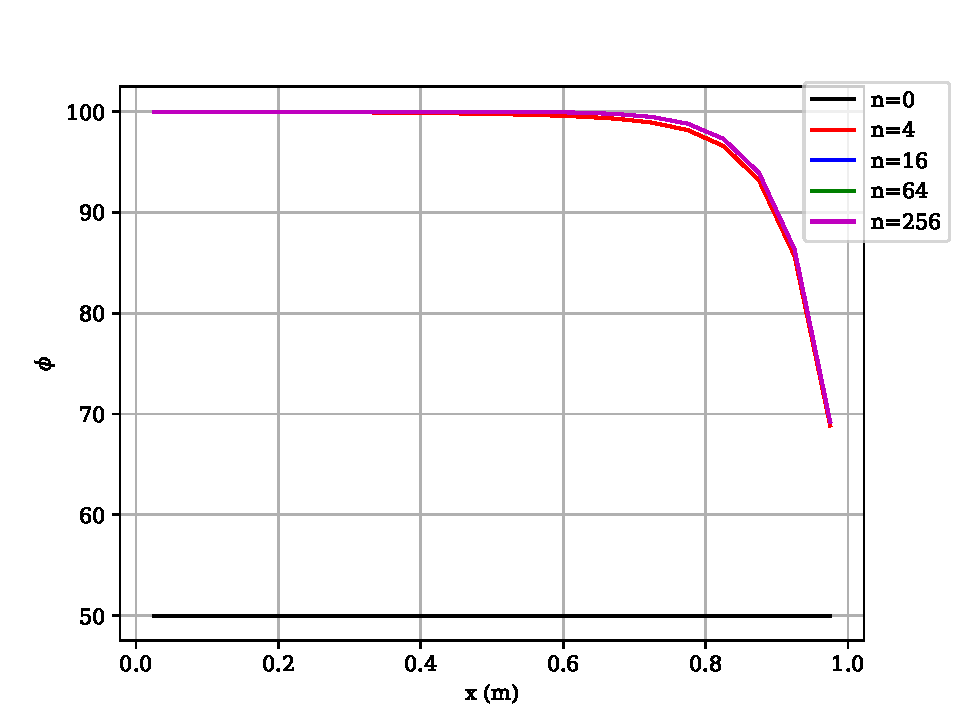
\includegraphics[width=\textwidth]{plots/graph_IE_case3.pdf}
    \caption{Implicit Euler solution for case 3: $K=20.0$.}
    \label{fig:ie3}
\end{figure}


Norm:
\begin{table}[htbp]
	 \centering
	 \caption{Norm values for Implicit Euler.}
	 \begin{tabular}{cc}
		 \toprule
		 $K$ & Norm \\ 
		 \midrule 
		 0.2 & 1.5567368462357045 \\ 
		 2.0 & 1.5504768792236276 \\ 
		 20.0 & 1.5504768792236157 \\ 
		 \bottomrule 
	 \end{tabular} 
	 \label{tab:error ie} 
\end{table}


\clearpage
\section{Discussion}


\clearpage
\section{Code}
\pythonexternal{code/main.py}


\end{document}